\chapter{Results}
\label{chap:results}

When an algorithm is being designed, its evaluation against existing solutions belongs to important stages of its development. This chapter describes this stage, informing about a data set used to debug and improve our solution, and the method of comparison with other solutions, such as fermi-kit and GATK. The last part of the chapter covers certain variants that proved to be interesting when examined by our algorithm.

\section{Test Data Set}
\label{sec:test-data-set}

The algorithm was tested on the first 40 megabases of chromosome 1 of the human genome. The test set is a high-coverage one and was obtained from the 1000 Genome Project. Except the input reads \cite{testreads}, variants called by fermi.kit and GATK are also available in form of VCF files \cite{testvcf}. The VCF files were used as a measure of algorithm quality. Since our algorithm also requires a reference sequence to work, we took the GRCh37 version \cite{testref}.

The input read set consists of 12475011 reads with lengh of 151 bases. Figure \ref{fig:test-kmer-frequency-distribution} shows k-mer frequency distribution of the set with k-mer size of 21 bases. The shape of the graph, when compared to Figure \ref{fig:kmer-frequency-distribution} suggests that the set contains read errors. Hence, an error correction step was applied.

\begin{figure}[h]
	\centering
	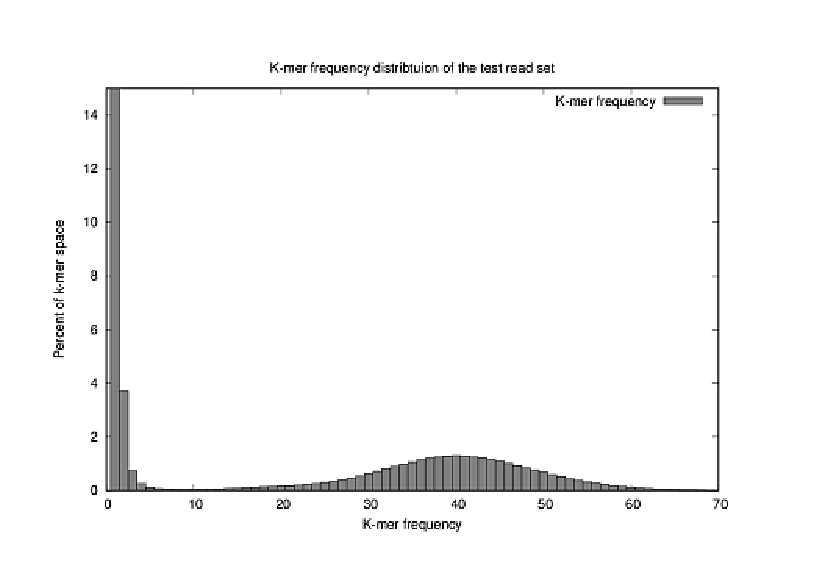
\includegraphics{img/test-kmer-frequency-distribution.pdf}
	\caption{K-mer frequency distrubtion of the raw input read set}
	\label{fig:test-kmer-frequency-distribution}
\end{figure}


As Table \ref{tab:test-correction} indicates, the error correction process removed and shortened certain amount of reads. About 21 \% of the input reads was subject to repairs. Figure \ref{fig:test-repair-frequency} shows a distribution of the number of repaired bases per read, not including effects of read shortage. It is clear, that about 21 \% of all reads received a base correction, and that, in most cases, only several bases were fixed. 

\begin{table}[h]
\begin{center}
\caption{Statistics related to error correction of the test data set}
\label{tab:test-correction}
\begin{tabular}{| c | c | p{5cm} |}
Category & Value & Percentage
\hline
Total reads & 12475011 & - \\
\hline
Removed & 64653 &  $0.52$ \% of all reads. \\
\hline
Shortened & 944 & $0.0076$ \% of all reads \\
\hline
Total bases & 1880123991 & - \\
\hline
Bases repaired & 5098764 &  $0.27$ of all bases \\
\hline
\end{tabular}
\end{table}

\begin{figure}[h]
	\centering
	\includegraphics{img/test-repair-frequency.ps}
	\caption{Distribution of a number of repaired bases in a single read}
	\label{fig:test-repair-frequency}
\end{figure}

Figure \ref{fig:test-kmer-frequency-distribution2} shows the k-mer frequency distribution of the corrected read set. Although quite far from perfect, the graph shape definitely resembles the ideal one better then in case of the raw  read set. 

\begin{figure}[h]
	\centering
	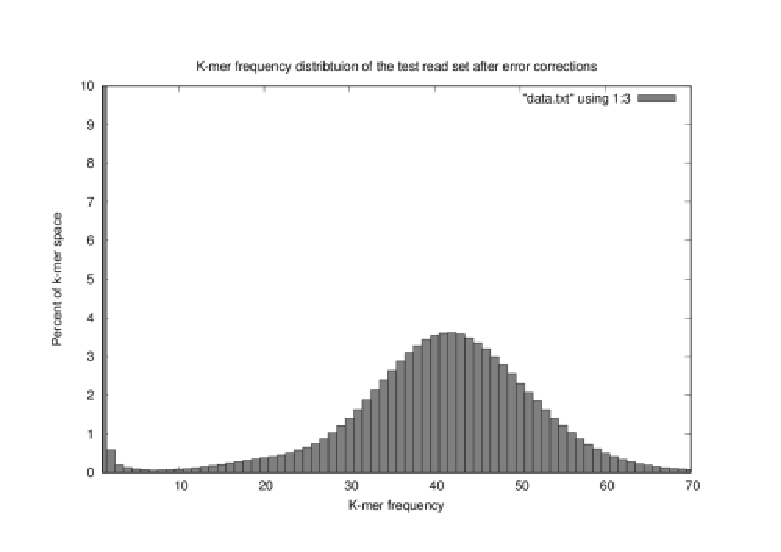
\includegraphics{img/test-kmer-frequency-distribution2.pdf}
	\caption{K-mer frequency distrubtion of the corrected read set}
	\label{fig:test-kmer-frequency-distribution2}
\end{figure}

As described in Section \ref{sec:data-preprocessing}, not all input reads, even from the corrected set, can be processed by our algorithm. Table \ref{tab:corrected-set-categories} summarizes numbers of reads unacceptable for various reasons. The preprocessing phase removed nearly one fifth of the corrected data set (18.99 \%). Most of the reads were removed due to being possible duplicates (87.65 \%). Quite a large portion of  reads were not accepted because of their low mapping quality (12.97 \%). Also, about 3 \% of all the reads were shortened in order to remove soft-clipped regions.

\begin{table}[h]
\begin{center}
\caption{Categories of reads present within the corrected test data set}
\label{tab:corrected-set-categories}
\begin{tabular}{| c | c | p{5cm} |}
\hline
Name & Value & Percentage \\
\hline
Total reads & 12410475 & - \\
\hline
Bad reads & 2357002  & $18.99$ \% of all reads \\
\hline
Low MAPQ & 305588 & $12.97$ \% of bad reads \\
\hline
Unmapped & 5020 & $0.21$ \% of bad reads \\
\hline
Supplementary & 33621 & $1.43$ \% of bad reads \\
\hline
Duplicate & 2065795 & $87.65$ \% of bad reads \\
\hline
Soft-clipped & 305209 & $3.04$ \% of accempted reads \\
\hline
\end{tabular}
\end{table}


\begin{itemize}
\item describe algorithms and software to evaluate the results (fermikit, fermikit run at individual regions, GATK, mpileup of samtools, rtgeval for evaluation),
\item Show the position-based and genotype results of rtgeval.
\item describe interesting variants (variants that are not found by other software, explain some false negatives, demonstrate that graph optimizations actually revealed some variants...).
\end{itemize}
